
\documentclass[a4paper,11pt]{article}
\usepackage[a4paper, margin=8em]{geometry}

% usa i pacchetti per la scrittura in italiano
\usepackage[french,italian]{babel}
\usepackage[T1]{fontenc}
\usepackage[utf8]{inputenc}
\frenchspacing 

% usa i pacchetti per la formattazione matematica
\usepackage{amsmath, amssymb, amsthm, amsfonts}

% usa altri pacchetti
\usepackage{gensymb}
\usepackage{hyperref}
\usepackage{standalone}

\usepackage{colortbl}

\usepackage{xstring}
\usepackage{karnaugh-map}

% imposta il titolo
\title{Appunti Calcolatori Elettronici}
\author{Luca Seggiani}
\date{2025}

% imposta lo stile
% usa helvetica
\usepackage[scaled]{helvet}
% usa palatino
\usepackage{palatino}
% usa un font monospazio guardabile
\usepackage{lmodern}

\renewcommand{\rmdefault}{ppl}
\renewcommand{\sfdefault}{phv}
\renewcommand{\ttdefault}{lmtt}

% circuiti
\usepackage{circuitikz}
\usetikzlibrary{babel}

% testo cerchiato
\newcommand*\circled[1]{\tikz[baseline=(char.base)]{
\node[shape=circle,draw,inner sep=2pt] (char) {#1};}}

% disponi il titolo
\makeatletter
\renewcommand{\maketitle} {
	\begin{center} 
		\begin{minipage}[t]{.8\textwidth}
			\textsf{\huge\bfseries \@title} 
		\end{minipage}%
		\begin{minipage}[t]{.2\textwidth}
			\raggedleft \vspace{-1.65em}
			\textsf{\small \@author} \vfill
			\textsf{\small \@date}
		\end{minipage}
		\par
	\end{center}

	\thispagestyle{empty}
	\pagestyle{fancy}
}
\makeatother

% disponi teoremi
\usepackage{tcolorbox}
\newtcolorbox[auto counter, number within=section]{theorem}[2][]{%
	colback=blue!10, 
	colframe=blue!40!black, 
	sharp corners=northwest,
	fonttitle=\sffamily\bfseries, 
	title=Teorema~\thetcbcounter: #2, 
	#1
}

% disponi definizioni
\newtcolorbox[auto counter, number within=section]{definition}[2][]{%
	colback=red!10,
	colframe=red!40!black,
	sharp corners=northwest,
	fonttitle=\sffamily\bfseries,
	title=Definizione~\thetcbcounter: #2,
	#1
}

% disponi codice
\usepackage{listings}
\usepackage[table]{xcolor}

\definecolor{codegreen}{rgb}{0,0.6,0}
\definecolor{codegray}{rgb}{0.5,0.5,0.5}
\definecolor{codepurple}{rgb}{0.58,0,0.82}
\definecolor{backcolour}{rgb}{0.95,0.95,0.92}

\lstdefinestyle{codestyle}{
	backgroundcolor=\color{black!5}, 
	commentstyle=\color{codegreen},
	keywordstyle=\bfseries\color{magenta},
	numberstyle=\sffamily\tiny\color{black!60},
	stringstyle=\color{green!50!black},
	basicstyle=\ttfamily\footnotesize,
	breakatwhitespace=false,         
	breaklines=true,                 
	captionpos=b,                    
	keepspaces=true,                 
	numbers=left,                    
	numbersep=5pt,                  
	showspaces=false,                
	showstringspaces=false,
	showtabs=false,                  
	tabsize=2
}

\lstdefinestyle{shellstyle}{
	backgroundcolor=\color{black!5}, 
	basicstyle=\ttfamily\footnotesize\color{black}, 
	commentstyle=\color{black}, 
	keywordstyle=\color{black},
	numberstyle=\color{black!5},
	stringstyle=\color{black}, 
	showspaces=false,
	showstringspaces=false, 
	showtabs=false, 
	tabsize=2, 
	numbers=none, 
	breaklines=true
}


\lstdefinelanguage{assembler}{ 
	keywords={AAA, AAD, AAM, AAS, ADC, ADCB, ADCW, ADCL, ADD, ADDB, ADDW, ADDL, AND, ANDB, ANDW, ANDL,
		ARPL, BOUND, BSF, BSFL, BSFW, BSR, BSRL, BSRW, BSWAP, BT, BTC, BTCB, BTCW, BTCL, BTR, 
		BTRB, BTRW, BTRL, BTS, BTSB, BTSW, BTSL, CALL, CBW, CDQ, CLC, CLD, CLI, CLTS, CMC, CMP,
		CMPB, CMPW, CMPL, CMPS, CMPSB, CMPSD, CMPSW, CMPXCHG, CMPXCHGB, CMPXCHGW, CMPXCHGL,
		CMPXCHG8B, CPUID, CWDE, DAA, DAS, DEC, DECB, DECW, DECL, DIV, DIVB, DIVW, DIVL, ENTER,
		HLT, IDIV, IDIVB, IDIVW, IDIVL, IMUL, IMULB, IMULW, IMULL, IN, INB, INW, INL, INC, INCB,
		INCW, INCL, INS, INSB, INSD, INSW, INT, INT3, INTO, INVD, INVLPG, IRET, IRETD, JA, JAE,
		JB, JBE, JC, JCXZ, JE, JECXZ, JG, JGE, JL, JLE, JMP, JNA, JNAE, JNB, JNBE, JNC, JNE, JNG,
		JNGE, JNL, JNLE, JNO, JNP, JNS, JNZ, JO, JP, JPE, JPO, JS, JZ, LAHF, LAR, LCALL, LDS,
		LEA, LEAVE, LES, LFS, LGDT, LGS, LIDT, LMSW, LOCK, LODSB, LODSD, LODSW, LOOP, LOOPE,
		LOOPNE, LSL, LSS, LTR, MOV, MOVB, MOVW, MOVL, MOVSB, MOVSD, MOVSW, MOVSX, MOVSXB,
		MOVSXW, MOVSXL, MOVZX, MOVZXB, MOVZXW, MOVZXL, MUL, MULB, MULW, MULL, NEG, NEGB, NEGW,
		NEGL, NOP, NOT, NOTB, NOTW, NOTL, OR, ORB, ORW, ORL, OUT, OUTB, OUTW, OUTL, OUTSB, OUTSD,
		OUTSW, POP, POPL, POPW, POPB, POPA, POPAD, POPF, POPFD, PUSH, PUSHL, PUSHW, PUSHB, PUSHA, 
		PUSHAD, PUSHF, PUSHFD, RCL, RCLB, RCLW, MOVSL, MOVSB, MOVSW, STOSL, STOSB, STOSW, LODSB, LODSW,
		LODSL, INSB, INSW, INSL, OUTSB, OUTSL, OUTSW
		RCLL, RCR, RCRB, RCRW, RCRL, RDMSR, RDPMC, RDTSC, REP, REPE, REPNE, RET, ROL, ROLB, ROLW,
		ROLL, ROR, RORB, RORW, RORL, SAHF, SAL, SALB, SALW, SALL, SAR, SARB, SARW, SARL, SBB,
		SBBB, SBBW, SBBL, SCASB, SCASD, SCASW, SETA, SETAE, SETB, SETBE, SETC, SETE, SETG, SETGE,
		SETL, SETLE, SETNA, SETNAE, SETNB, SETNBE, SETNC, SETNE, SETNG, SETNGE, SETNL, SETNLE,
		SETNO, SETNP, SETNS, SETNZ, SETO, SETP, SETPE, SETPO, SETS, SETZ, SGDT, SHL, SHLB, SHLW,
		SHLL, SHLD, SHR, SHRB, SHRW, SHRL, SHRD, SIDT, SLDT, SMSW, STC, STD, STI, STOSB, STOSD,
		STOSW, STR, SUB, SUBB, SUBW, SUBL, TEST, TESTB, TESTW, TESTL, VERR, VERW, WAIT, WBINVD,
	XADD, XADDB, XADDW, XADDL, XCHG, XCHGB, XCHGW, XCHGL, XLAT, XLATB, XOR, XORB, XORW, XORL},
	keywordstyle=\color{blue}\bfseries,
	ndkeywordstyle=\color{darkgray}\bfseries,
	identifierstyle=\color{black},
	sensitive=false,
	comment=[l]{\#},
	morecomment=[s]{/*}{*/},
	commentstyle=\color{purple}\ttfamily,
	stringstyle=\color{red}\ttfamily,
	morestring=[b]',
	morestring=[b]"
}

\lstset{language=assembler, style=codestyle}

% disponi sezioni
\usepackage{titlesec}

\titleformat{\section}
{\sffamily\Large\bfseries} 
{\thesection}{1em}{} 
\titleformat{\subsection}
{\sffamily\large\bfseries}   
{\thesubsection}{1em}{} 
\titleformat{\subsubsection}
{\sffamily\normalsize\bfseries} 
{\thesubsubsection}{1em}{}

% tikz
\usepackage{tikz}

% float
\usepackage{float}

% grafici
\usepackage{pgfplots}
\pgfplotsset{width=10cm,compat=1.9}

% disponi alberi
\usepackage{forest}

\forestset{
	rectstyle/.style={
		for tree={rectangle,draw,font=\large\sffamily}
	},
	roundstyle/.style={
		for tree={circle,draw,font=\large}
	}
}

% disponi algoritmi
\usepackage{algorithm}
\usepackage{algorithmic}
\makeatletter
\renewcommand{\ALG@name}{Algoritmo}
\makeatother

% disponi numeri di pagina
\usepackage{fancyhdr}
\fancyhf{} 
\fancyfoot[L]{\sffamily{\thepage}}

\makeatletter
\fancyhead[L]{\raisebox{1ex}[0pt][0pt]{\sffamily{\@title \ \@date}}} 
\fancyhead[R]{\raisebox{1ex}[0pt][0pt]{\sffamily{\@author}}}
\makeatother

\begin{document}
% sezione (data)
\section{Lezione del 28-04-25}

% stili pagina
\thispagestyle{empty}
\pagestyle{fancy}

% testo
\subsection{DMA}
Vediamo di introdurre il meccanismo del \textbf{DMA} (\textit{Direct Memory Access}).

Finora l'accesso a periferiche era fatto a \textit{controllo programma} o \textit{controllo interruzione}.
Chiaramente il controllo programma era più veloce, in quanto il programma provvedeva a trasferire ogni byte immediatamente appena l'interfaccia era pronta, mentre nel controllo interruzione bisognava prima eseguire tutti i passaggi necessari all'esecuzione degli \textit{handler} per portare in esecuzione il processo esterno, ecc... 

Introduciamo quindi il DMA per delegare tutta l'operazione di trasferimento dati dalle interfacce alle interfacce stesse.
Vorremo quindi avere delle primitive:
\begin{itemize}
	\item \lstinline|read_n|, trasferimento da interfaccia a RAM di un buffer $[b, b + n)$;
	\item \lstinline|write_n|, trasferimento da RAM a interfaccia di un buffer $[b, b+n)$.
\end{itemize}

Se è l'interfaccia stessa a compiere l'operazione di trasferimento, al processore servirà nuovamente un modo di controllare l'esito dell'operazione, che potra essere ancora a \textit{controllo programma} o a \textit{controllo interruzione} (che è il caso più comune).

Aggiungiamo quindi un \textbf{controllore DMA} al bus visto finora.
Questo sarà di base dotato di due registri, uno per il buffer corrente (\textbf{B}) e uno per la sua dimensione (\textbf{N}), e potrà accedere in lettura e scrittura allo spazio di memoria al pari di come farebbe la CPU.
Notiamo che non c'è bisogno che la RAM distingua fra operazioni effettuate da CPU o DMA, in quanto per questa sono equivalenti.

Dotiamo quindi il controllore DMA di due linee di handshake \lstinline|HOLD| e \lstinline|HOLDA| che lo connettono alla CPU:

\begin{center}
	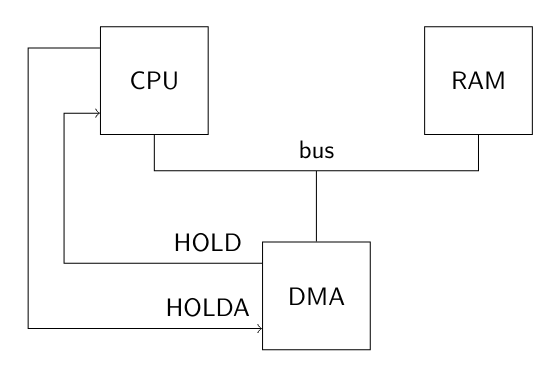
\includegraphics[scale=0.5]{../figures/dma_base.png}
\end{center}

Al momento dell'inizio di un'operazione DMA, il controllore alza \lstinline|HOLD|, e la CPU risponde alzando \lstinline|HOLDA| e portando i suoi pin di uscita in alta impedenza.
Da qui in poi il controllore lavora sul bus, in regime di \lstinline|cycle-stealing|, cioè "rubando" cicli di accesso alla CPU.
Finita l'operazione, il controllore abbassa nuovamente \lstinline|HOLD|, a cui la CPU risponde abbassando \lstinline|HOLDA| e riprendendo a scrivere sul bus.

Storicamente questo meccanismo era utile per interfacce più veloci della CPU stessa (così era la RAM, ed erano ad esempio i controllori video, che si dividevano circa la metà del tempo RAM con la CPU).
Oggi, lo stesso discorso vale nel senso opposto, ad esempio per le interfacce di rete, che raggiungono velocità del Gigabit al secondo (quindi molto più veloci della CPU).

\subsubsection{DMA e cache}
Vediamo di reintrodurre nel bus così modificato la cache.
Innanzitutto, i contendenti al bus non saranno più CPU e controllore DMA, ma cache e controllore DMA, per cui le linee di \lstinline|HOLD| e \lstinline|HOLDA| saranno fra questi due:

\begin{center}
	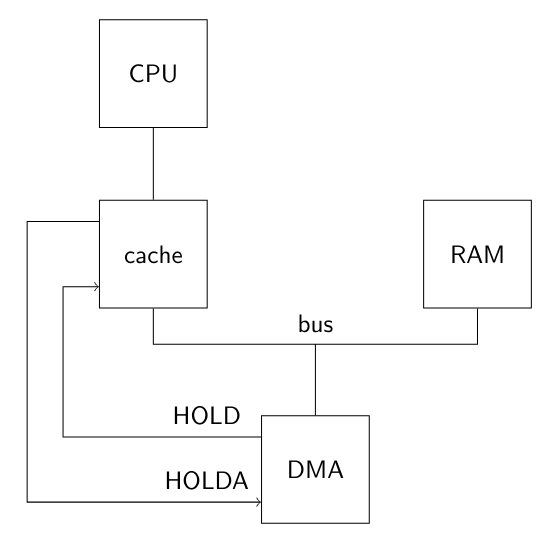
\includegraphics[scale=0.5]{../figures/dma_cache.png}
\end{center}

Il vantaggio immediato che abbiamo è che probabilmente la maggior parte dei dati necessari alla CPU saranno in cache, per cui il regime di cycle-stealing non sarà troppo dannoso all'attività della CPU (ricordiamo che la cache accede al bus solamente quando si ha una \textit{miss}).

Un problema potrebbe invece essere che la cache potrebbe perdersi gli aggiornamenti effettuati dal controllore DMA.
Vediamo nel dettaglio quali problemi possono apparire, e quali soluzioni si possono adottare. in regime di \textit{write-through} e \textit{write-back}.

\par\smallskip
\noindent
\textbf{\sffamily{Write-through}} \\
Supponiamo quindi come primo esempio che la cache adotti una politica \textit{write-through}, e che chiaramente il programmatore si impegni a non toccare il buffer per tutto il tempo del trasferimento.

\begin{itemize}
	\item 
		In questo caso, per operazioni di scrittura su dispositivo non ci saranno problemi, in quanto la politicha write-trough mantiene sia la RAM che la cache in uno stato identico e consistente, e il controllore DMA non modifica la RAM in operazioni di uscita.
	\item
		Viceversa, per operazioni di lettura da dispositivo avremo problemi, in quanto potremmo intaccare una zona di memoria che era replicata in cache, e la cache non avrà modo di conoscere tale aggiornamento.

		Per ovviare a tale problema abbiamo effettivamente due soluzioni:
		\begin{itemize}
			\item La prima soluzione è \textit{lato hardware}, e consiste nel dotare la cache della possibilità di fare \textit{snooping} del bus, cioè capire a quali indirizzi il DMA sta accedendo, farne un lookup esattamente nella maniera in cui si farebbe lookup degli indirizzi richiesti dalla CPU, e procedere ricopiando i dati modificati (\textit{snarfing}) o direttamente invalidando tale porzione di cache (soluzione adottata dall'architettura Intel x86);
			\item La seconda soluzione è \textit{lato software}, e consiste nell'introdurre un'apposita istruzione per forzare il controllore di cache ad effettuare l'invalidazione di cache.
				Utilizzeremo quindi questa istruzione per invalidare i buffer forniti per la lettura da dispositivo al DMA, idealmente alla fine dell'operazione di trasferimento.

				Nel frattempo chiaramente non vorremmo toccare nessuna delle cacheline impegnate dal buffer, che possono definire una regione anche maggiore in dimensioni del buffer stesso.
				L'invalidazione a termine operazione viene effettuata a fine operazione proprio per questo motivo, ma una soluzione alternativa potrebbe anche essere l'adottare buffer allineati ai 64 KiB delle cacheline.
		\end{itemize}
\end{itemize}

\par\smallskip
\noindent
\textbf{\sffamily{Write-back}} \\
Fatta invece l'ipotesi di \textit{write-back}, cioè di scritture effettuate in differita dalla cache alla RAM da parte del controllore di cache, che mantiene le modifiche temporaneamente nella sua memoria, avremo problemi sia in lettura che in scrittura.

\begin{itemize}
	\item 
		In scrittura su dispositivo avremo chiaramente che il buffer in RAM potrebbe non essere stato aggiornato con le modifiche in cache al momento dell'inizio dell'operazione da parte del controllore DMA.
		\begin{itemize}
			\item Qui la soluzione \textit{lato hardware} è di definire un protocollo per cui il controllore DMA deve prima parlare con la cache, fornendo l'indirizzo a cui intende accedere (questa fase viene detta sempre di \textit{snooping}).
				In questo caso la cache ha il tempo di controllare l'indirizzo e quindi capire se la cacheline corrispondente è \textit{dirty}, e quindi in RAM ce n'è una versione obsoleta.
				A questo punto potrà agire di conseguenza, fornendo lei stessa i dati aggiornati o effettuando una write-back;
			\item La soluzione \textit{lato software} sarà invece di fornire un'istruzione di pulizia, che permetta di forzare il write-back delle cacheline coinvolte nel buffer prima di iniziare l'operazione di lettura in RAM da parte del controllore DMA.
		\end{itemize}
	\item
		In lettura da dispositivo avremo invece che il controllore DMA potrebbe intaccare zone di memoria per cui la cache stava pianificando scritture in differita.
		\begin{itemize}
			\item In questo caso il chipset PIIX3 emulato da QEMU, ad esempio, ottiene dalla cache la versione più aggiornata, che viene invalidata (se questa esiste in cache), effettua il \textit{merge} fra questa e quanto ottenuto dal dispositivo internamente al controllore DMA, che provvede poi ad effettuare la scrittura in RAM;
				Per cacheline complete, abbiamo che il DMA può adottare anche il protocollo \textit{write invalidate}, per cui la cache attraverso un'operazione di snooping può verificare che un intera cacheline è stata modificata e limitarsi ad invalidarla: ci si aspetterà che il controllore DMA la modificherà integralmente e non ci sarà bisogno di merge;
			\item La stessa istruzione di pulizia di cui abbiamo parlato nel caso precedente vale anche per risolvere questo problema \textit{lato software}, sempre prima dell'operazione di trasferimento (in modo che la versione dei dati in RAM sia la più recente, cioè quella ottenuta dal controllore DMA).
		\end{itemize}
\end{itemize}

\subsubsection{DMA e MMU}
Reintroduciamo infine la MMU.
Qui il problema sarà chiaramente che la CPU conoscerà indirizzi virtuali, mentre la DMU avrà bisogno di indirizzi fisici.

Far passare la DMU attraverso la MMU non sarà una soluzione, in quanto non possiamo essere sicuri che durante l'operazione di trasferimento l'albero di traduzione resta lo stesso.

Abbiamo quindi che il problema dovrà essere risolto lato software, passando al controllore DMA direttamente indirizzi fisici, attraverso la finestra FM.
A questo punto però non potremmo aspettarci il corretto trasferimento di regioni di memoria di dimensione superiore a quella di una pagina, in quanto il controllore DMA non ha modo di capire quando passare da una pagina all'altra, o dove queste pagine siano in primo luogo.

Vogliamo quindi che i buffer che passiamo al controllore DMA non superino i confini di una pagina, e saremo quindi costretti a segmentare buffer che passano per più confini.

\par\smallskip

Infine, vorremo che il kernel si impegni a mantenere costante l'impiego delle regioni di memoria dedicate ai buffer forniti al controllore DMA, cioè non effettui swap in o swap out dei processi che li forniscono mentre l'operazione di trasferimento è ancora in corso, in quanto il controllore non ha modo di rilevare tali variazioni e potrebbe continuare operazioni di scrittura o lettura con effetti disastrosi.

\subsubsection{DMA nel bus PCI}
Inseriamo quindi il controllore DMA nel bus PCI.

In questo caso sarà il ponte ospite-PCI ad occuparsi del DMA sul bus principale, secondo le regole e le linee di connessione col controllore di cache appena viste.

Avremo quindi bisogno che nei singoli bus PCI ogni interfaccia abbia la possibilità di prendere il controllo del bus, secondo il cosiddetto meccanismo di \textbf{bus mastering} (avevamo già visto come ogni interfaccia, e anzi più propriamente ogni \textit{funzione} PCI poteva iniziare transazioni sul bus PCI nella sezione 18.1).

\noindent
\begin{minipage}{\textwidth}

	Il bus mastering nei bus PCI viene gestito da un \textbf{arbitro}, che è collegato con linee \lstinline|REQ| e \lstinline|GNT| ad ogni interfaccia:

	\begin{center}
		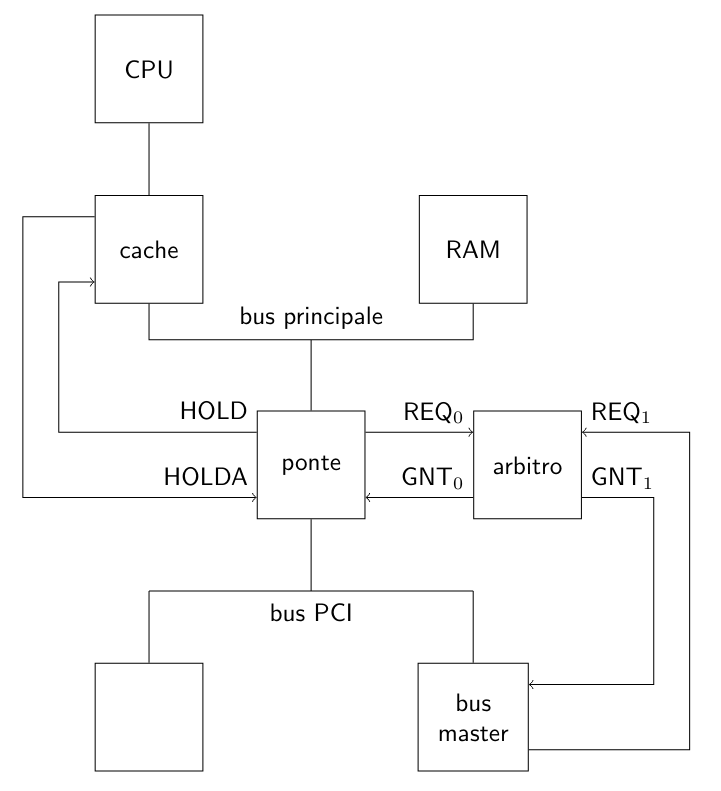
\includegraphics[scale=0.55]{../figures/dma_pci.png}
	\end{center}

\end{minipage}

Le interfacce richiedono quindi accesso al bus attraverso la \lstinline|REQ|, mentre questo gli risponde attraverso la \lstinline|GNT|.
Una volta ottenuta la conferma su \lstinline|GNT|, il dispositivo in bus mastering può comportarsi come se si trovasse sul bus principale (passando attraverso il ponte ospite-PCI).
Le operazioni che questo svolge potranno essere poi \textit{bufferizzate} dal ponte ospite-PCI, cioè questo potrà memorizzare le modifiche in RAM ottenute lato bus PCI, per poi riportarle in differita alla RAM vera e propria.

Questo ultimo dettaglio potrebbe dare dei problemi per quanto riguarda la sincronizzazione fra interfacce e CPU, in quanto un'interfaccia potrebbe inviare un segnale di termine operazione attraverso l'APIC, quando essa \textit{crede} l'operazione sia finita (e lo farà perche lato bus PCI questa effettivamente lo è), mentre lato bus locale il ponte non ha ancora attualizzato i dati in RAM.
La soluzione  sarà quella di collegare l'APIC al ponte, in modo da poter ritardare le interruzioni esterne alla fine delle operazioni di trasferimento.

Infine, possiamo anticipare che nei processori moderni gli interrupt si inviano attraverso scritture in regioni specifiche di memoria, che l'apparato CPU riconosce autonomamente come interruzione.
Questo corrisponde in un delay naturale fra i trasferimenti e l'invio di interruzioni da una stessa interfaccia.

Notiamo che entrambe le soluzioni richiedono che il ponte adotti una politica strettamente FIFO alla gestione dei trasferimenti: il primo trasferimento iniziato e completato lato bus PCI è il primo trasferimento a essere riportato dal buffer interno al ponte in RAM.

\end{document}
